\documentclass[11pt]{article}
\usepackage[T1]{fontenc}
\usepackage[utf8]{inputenc}
\usepackage{lmodern,microtype}
\input{glyphtounicode}
\input{glyphtounicode-cmex}
\pdfglyphtounicode{vextendsingle}{007C}
\pdfglyphtounicode{vextenddouble}{2016}
\pdfgentounicode=1
\usepackage[margin=1in]{geometry}
\usepackage{amsmath,amssymb,amsthm,mathtools}
\usepackage{enumitem,graphicx,xcolor,flafter,xurl,needspace}
\usepackage{tikz}
\usetikzlibrary{arrows.meta,calc,patterns}
\usepackage[numbers,sort&compress]{natbib}
\usepackage[colorlinks=true,linkcolor=blue!45!black,citecolor=blue!45!black,
 urlcolor=blue!45!black,
 pdftitle={The symmetric Mahler conjecture and its equality cases},
 pdfauthor={OpenAI}]{hyperref}
\newtheorem{theorem}{Theorem}[section]
\newtheorem{lemma}[theorem]{Lemma}
\newtheorem{proposition}[theorem]{Proposition}
\newtheorem{corollary}[theorem]{Corollary}
\theoremstyle{definition}
\newtheorem{definition}[theorem]{Definition}
\newtheorem{remark}[theorem]{Remark}
\newcommand{\R}{\mathbb R}
\newcommand{\C}{\mathbb C}
\newcommand{\D}{\mathbb D}
\newcommand{\ddc}{dd^c}
\DeclareMathOperator{\conv}{conv}
\setlength{\emergencystretch}{1.5em}
\setcounter{tocdepth}{2}
\renewcommand{\topfraction}{0.85}
\renewcommand{\textfraction}{0.1}
\renewcommand{\floatpagefraction}{0.8}
\title{The symmetric Mahler conjecture and its equality cases}
\author{OpenAI}
\date{September 22, 2026}
\begin{document}
\maketitle
\begin{abstract}
We resolve the symmetric Mahler conjecture positively, including its
equality classification. Every origin-symmetric convex body in $\R^n$ has volume
product at least $4^n/n!$, with equality exactly for invertible linear
images of Hanner polytopes.
\end{abstract}
\tableofcontents
\section{Introduction}\label{sec:introduction}

A convex body is a compact convex subset of $\R^n$ with nonempty
interior. If $K=-K$, its center $0$ is an interior point, and its
polar body is
\[
 K^\circ=\{y\in\R^n:\langle x,y\rangle\le1
                         \text{ for every }x\in K\}.
\]
Write $|K|$ for $n$-dimensional Lebesgue volume and
$P(K)=|K|\,|K^\circ|$ for the volume product. The two determinant
factors cancel under an invertible linear change of coordinates, so
$P(TK)=P(K)$. Mahler's symmetric volume-product problem asks how small
this linear invariant can be. The conjectured value is $4^n/n!$,
the product of a cube and its polar cross-polytope. We prove this bound
in every dimension and classify the equality cases.

The extremal bodies are defined recursively. A centered nondegenerate
interval is a one-dimensional \emph{Hanner polytope}. Given Hanner
polytopes $H_1\subset\R^k$ and $H_2\subset\R^l$, their Cartesian
product and the convex hull
\[
 \begin{aligned}
 H_1\oplus_\infty H_2&=H_1\times H_2,\\
 H_1\oplus_1 H_2&=
 \conv\bigl((H_1\times\{0\})\cup(\{0\}\times H_2)\bigr)
 \end{aligned}
\]
are Hanner polytopes in $\R^{k+l}$. These are the $\ell_\infty$ and
$\ell_1$ sums, respectively. This class contains cubes, cross-polytopes,
and mixed recursive sums. We call an invertible linear image of a
Hanner polytope a \emph{linear Hanner body}.

\begin{theorem}\label{thm:main}
For every integer $n\ge1$ and every origin-symmetric convex body
$K\subset\R^n$,
\begin{equation}\label{eq:main-inequality}
 |K|\,|K^\circ|\ge\frac{4^n}{n!}.
\end{equation}
Equality holds if and only if $K$ is a linear Hanner body.
\end{theorem}

The linear equivalence in the statement respects the fixed origin
used for polarity.

\subsection{History and context}

Mahler introduced the volume-product problem in his work on convex
bodies and transference in the geometry of numbers~\cite{Mahler1939};
the planar inequality also goes back to him~\cite{MahlerPlanar1939}.
Reisner later characterized its equality cases as parallelograms,
as a consequence of his zonoid theorem~\cite[p.~340]{Reisner1986}.
Iriyeh and Shibata proved the complete three-dimensional symmetric
theorem, including equality~\cite[Theorem~1.1]{IriyehShibata}.
Fradelizi, Hubard, Meyer, Rold\'an-Pensado, and Zvavitch gave a
shorter proof based on equipartitions, together with another equality
argument and stability~\cite{FradeliziHubardMeyerRoldanZvavitch2022}.
Chen, Li, Xi, and Xu recently gave a shadow-flow proof of that theorem
in a preprint that also treats the nonsymmetric three-dimensional
problem~\cite[Theorem~7.1]{ChenLiXiXu2026}.

Hanner's recursively constructed spaces~\cite{Hanner1956} already
play a central role in the known higher-dimensional cases.
Saint-Raymond proved the sharp inequality for unconditional bodies
(those invariant under coordinate sign changes)~\cite{SaintRaymond1981};
Meyer and Reisner identified the Hanner equality cases in that
class~\cite{Meyer1986,Reisner1987}. Reisner also proved the sharp
inequality for zonoids, which are Hausdorff limits of Minkowski sums of
centered segments, and showed that equality within that class means a
parallelotope~\cite{Reisner1985,Reisner1986}; Gordon, Meyer, and
Reisner later gave a short geometric proof~\cite{GordonMeyerReisner1988}.
For local questions in Banach--Mazur distance, Nazarov, Petrov,
Ryabogin, and Zvavitch established strict local minimality, up to
linear equivalence, of the cube~\cite{NazarovPetrovRyaboginZvavitch2010}.
Kim extended this to all Hanner polytopes~\cite{Kim2014}.
Kim and Zvavitch obtained stability
in the unconditional class and the inequality in a neighborhood of
that class~\cite{KimZvavitch2015}.

A separate line of work seeks dimension-independent exponential
bounds without the sharp constant. Bourgain and Milman established
such a reverse Blaschke--Santal\'o inequality~\cite{BourgainMilman};
Kuperberg obtained an explicit stronger bound by a geometric argument
using Gauss linking integrals~\cite{Kuperberg}. Complex-analytic
approaches provide another setting for these questions. Nazarov used
H\"ormander's $\bar\partial$ theorem and Bergman kernels for the
reverse Blaschke--Santal\'o inequality~\cite{Nazarov2012}.
Berndtsson recast Kuperberg's proof using complex integrals
\cite{Berndtsson}. In a symplectic approach, Karasev proved the sharp
inequality for hyperplane sections and projections of $\ell_p$ balls
($1\le p\le\infty$) and Hanner polytopes~\cite[Theorems~4.2 and~4.4]{Karasev}.
These works give analytic and geometric precedents for volume-product
estimates; their estimates are not hypotheses of our proof.

The analytic ingredient is a conformal map of the disk for which
uniform angular measure on the boundary maps to a uniform imaginary
coordinate. It is a rotation of
Gross's example for the uniform distribution in his conformal Skorokhod
embedding~\cite[Section~3.2]{Gross}. A holomorphic mass estimate turns
that boundary law into a lower bound for an integral of feasible-simplex
volumes over the primal body. We prove the mass estimate directly by
Stokes' theorem, with its precise normalization; its general background
is the theory of generalized Lelong numbers~\cite[Sections~3 and~5]{Demailly}.
The symmetric-convex extremal-function framework of Lundin and Baran
was a further motivation for the analytic search; see
\cite{Lundin1985} and the formula recorded in
\cite[Proposition~1.2, pp.~246--247]{BosCalviLevenberg2001}.
The proof here instead uses the direct isolated-zero mass calculation,
not those extremal-function formulas as premises.
The equality argument leads to a classical property of normed spaces:
any three pairwise-intersecting closed balls have a common point.
Hanner studied the associated recursively constructed convex bodies
\cite{Hanner1956}. Lima's norm-additive decomposition criterion
\cite[Theorem~1.2]{Lima1978}, also recorded in
Hansen--Lima~\cite[Theorem~3.6(4)]{HansenLima1981}, is exactly the
metric-median condition used below. Reisner's unconditional equality
theorem already connects minimal volume product to this ball
intersection structure~\cite[Theorem~1]{Reisner1987}. Our endpoint
argument obtains the structure without assuming unconditionality;
Hansen--Lima's finite-dimensional classification is the final input
\cite[Corollary~7.4]{HansenLima1981}.

For a body without a prescribed center, the general Mahler problem
instead minimizes $|K|\,|(K-z)^\circ|$ over $z\in\operatorname{int}K$.
Its conjectured constant $(n+1)^{n+1}/(n!)^2$ is smaller than the
symmetric constant for $n\ge2$; a result for that general problem alone
therefore does not establish Theorem~\ref{thm:main}. The argument here
uses symmetry throughout and is independent of the general theorem
proved in the companion paper
\cite[Theorem~1.1]{OpenAIGeneralMahler2026}.

\subsection{Proof overview}

Section~\ref{sec:convex} records polarity and the two norm-sum formulas.
They show that every Hanner body has the stated volume product.
The remaining work is the lower bound and its converse equality
statement.

First let
\[
 A=\{X\in\R^d:|b_i\cdot X|\le1,\ 1\le i\le m\},
 \qquad A^\circ=\conv\{\pm b_1,\ldots,\pm b_m\},
\]
where the nonzero, pairwise nonproportional rows $b_i$ span $\R^d$.
Section~\ref{sec:lens} constructs
a planar lens with horizontal half-width $\lambda(t)$ at height $t$.
For $X\in\operatorname{int}A$, use this width to form
\[
 L_X=\{Y\in\R^d:|b_i\cdot Y|\le\lambda(b_i\cdot X),\ 1\le i\le m\}.
\]
Each independent $d$-tuple of signed constraints that are tight at
one point of $L_X$ determines a simplex: take the convex hull of $0$
and those signed rows. Let $\Sigma_X$ be the union of these simplices.
It lies in $A^\circ$.

Write $F$ for the conformal map from the unit disk to the lens.
For each set $I$ of $d$ independent rows, sample independent uniform angles
$\theta_i$ and solve $b_iZ=F(e^{i\theta_i})$, $i\in I$, for the
complex vector $Z$. Let $P_I$ be the probability that all remaining
row coordinates also lie in the closed lens. Section~\ref{sec:feasibility}
applies the mass estimate of Section~\ref{sec:holomorphic-mass} to high
powers of the inverse map: after a change of radial variables, the
Jacobian integrals concentrate on these boundary samples and force
$S:=\sum_I P_I\ge1$.
The uniform imaginary coordinate then identifies this probability sum
with the simplex integral in Section~\ref{sec:simplex}:
\[
 1\le S=\frac{d!}{4^d}\int_A|\Sigma_X|\,dX
                    \le\frac{d!}{4^d}|A|\,|A^\circ|.
\]
The first inequality is analytic; the last is the inclusion just
described. The exact identity behind this bound also controls the
missing volume $|A^\circ|-|\Sigma_X|$. Approximation extends the
inequality to all origin-symmetric convex bodies.

For equality, set $Q=K^\circ$ and pass to the body
\[
 B=K\oplus_1[-1,1],\qquad B^\circ=Q\times[-1,1]
\]
in dimension $d=n+1$. The norm-sum formula preserves equality at the
new dimension. Inner polytope approximations to $Q$ therefore have
integrated missing volume tending to zero. Section~\ref{sec:zero-deficit}
uses product neighborhoods to obtain, for each interior point of $B$
and each nonzero direction, a representation whose rows attain their
lens bounds at one vector satisfying all the constraints. This includes
degenerate limiting representations.
Finally, Section~\ref{sec:median} examines points approaching an apex
of $B$. The lens asymptotic gives a support-function inequality,
and convex separation gives a metric median for every triple in the
norm with unit ball $Q$: a point whose distances to each pair sum to
that pair's distance. The Hansen--Lima theorem then identifies $Q$,
and hence $K$, as a linear Hanner body
\cite[Corollary~7.4]{HansenLima1981}.

We next derive functional and entropy--transport consequences of the
all-dimensional theorem. The geometric proof begins in
Section~\ref{sec:convex} and ends in Section~\ref{sec:median}.

\subsection{Functional Mahler inequality}\label{sec:functional-mahler}

The volume-product problem has a functional form in which polarity is
replaced by convex conjugation. For a proper lower-semicontinuous convex
function $\varphi:\R^n\to\R\cup\{+\infty\}$, its Fenchel--Legendre transform is
\[
 \varphi^*(y)=\sup_{x\in\R^n}\{\langle x,y\rangle-\varphi(x)\},
 \qquad y\in\R^n.
\]
We use the convention $e^{-\infty}=0$.

\begin{corollary}[Even functional Mahler inequality]\label{cor:functional-mahler}
For every integer $n\ge1$ and every even proper lower-semicontinuous
convex function $\varphi:\R^n\to\R\cup\{+\infty\}$ such that
$0<\int_{\R^n}e^{-\varphi(x)}\,dx<\infty$,
\[
 \left(\int_{\R^n}e^{-\varphi(x)}\,dx\right)
 \left(\int_{\R^n}e^{-\varphi^*(y)}\,dy\right)\ge4^n.
\]
The second integral is allowed to be infinite, in which case the
inequality is immediate.
\end{corollary}

\begin{proof}
Set $f=e^{-\varphi}$, a nonzero integrable log-concave function. For
$z\in\R^n$, Fradelizi and Meyer use the polar function
\[
 f^z(y)=\inf_{\{x:f(x)>0\}}
        \frac{e^{-\langle x-z,y-z\rangle}}{f(x)}
\]
and the translation-minimized functional volume product
\[
 \mathcal P(f)=
 \left(\int_{\R^n}f(x)\,dx\right)
 \inf_{z\in\R^n}\int_{\R^n}f^z(y)\,dy.
\]
Their Proposition~1(a) states that the symmetric geometric Mahler
inequality in every dimension implies $\mathcal P(f)\ge4^n$ for every
even log-concave function on $\R^n$ with $0<\int_{\R^n}f<\infty$
\cite{FradeliziMeyer2008}. Theorem~\ref{thm:main} supplies this
all-dimensional hypothesis. Since $f^0=e^{-\varphi^*}$, the product
in Corollary~\ref{cor:functional-mahler} is at least $\mathcal P(f)$.
\end{proof}

The cited implication uses auxiliary convex bodies in dimensions
$n+m$ and lets $m$ tend to infinity; it is not an application only of
the geometric theorem in dimension $n$. The constant is sharp:
for $\varphi(x)=\sum_{i=1}^n|x_i|$, the transform $\varphi^*$ is zero on
$[-1,1]^n$ and $+\infty$ outside, and both integrals in
the corollary equal $2^n$. The equality classification
in Theorem~\ref{thm:main} concerns convex bodies. The limiting
implication does not by itself classify the even potentials for which
equality holds \cite[p.~1437]{FradeliziMeyer2008}.

For potentials without evenness, the companion paper on general convex
bodies gives the sharp lower bound $e^n$
\cite[Corollary~1.2]{OpenAIGeneralMahler2026}.

The functional inequality also has an entropy--transport formulation.
For a log-concave probability measure $\eta$ with a density, let
$H(\eta)=\int\log(d\eta/dx)\,d\eta$ denote its entropy relative to
Lebesgue measure, the negative of differential Shannon entropy.
For probability measures $\mu_1,\mu_2$ with finite first moments, set
\[
 \mathcal T(\mu_1,\mu_2)=
 \inf_{f\in\mathcal F}\left\{\int f\,d\mu_1+\int f^*\,d\mu_2\right\},
\]
where $\mathcal F$ is the class of proper lower-semicontinuous convex
functions $\R^n\to\R\cup\{+\infty\}$ and $f^*$ is the Fenchel--Legendre
transform. The cost $\mathcal T$ is allowed to be $+\infty$.

\begin{corollary}[Symmetric entropy--transport inequality]\label{cor:entropy-transport}
For every integer $n\ge1$, let $\eta_i(dx)=e^{-V_i(x)}\,dx$, $i=1,2$,
be full-dimensional log-concave probability measures, both symmetric
about the origin, with proper lower-semicontinuous convex potentials
$V_i$. Suppose their densities are essentially continuous, meaning that
$e^{-V_i}=0$ at $\mathcal H^{n-1}$-almost every point of
$\partial\operatorname{supp}\eta_i$. Their moment measures
$\nu_i=(\nabla V_i)_\#\eta_i$ have finite first moments,
$H(\eta_i)=-\int V_i\,d\eta_i$ is finite, and
\[
 H(\eta_1)+H(\eta_2)\le -n\log(4e^2)+\mathcal T(\nu_1,\nu_2).
\]
\end{corollary}

\begin{proof}
For $\rho_i=e^{-V_i}$, the identity
$|\nabla\rho_i|=|\nabla V_i|e^{-V_i}$ holds almost everywhere on the
interior of the support. Lemma~4 and the proof of Proposition~7 of
\cite{CorderoErausquinKlartag2015} give
$\int |\nabla\rho_i|<\infty$ and $V_i\in L^1(\eta_i)$, respectively.
The pushforward definition of $\nu_i$ therefore gives its finite first
moment, and $H(\eta_i)=-\int V_i\,d\eta_i$ is finite.
Gozlan's equivalence between the symmetric functional inverse Santal\'o
and entropy--transport inequalities, as stated in
\cite[Theorem~1.3]{FradeliziGozlanZugmeyer2021}, applies to
Corollary~\ref{cor:functional-mahler} with $c=4$.
\end{proof}

\section{Polarity, norm sums, and Hanner polytopes}\label{sec:convex}

All bodies below are symmetric about the origin. In addition to the
polar and volume product defined in Section~\ref{sec:introduction}, we use
the gauge and support function
\[
 p_A(x)=\inf\{t>0:x\in tA\},\qquad
 h_A(y)=\max_{x\in A}\langle x,y\rangle.
\]
Dual spaces are identified with Euclidean coordinate spaces, and
$|A|$ always denotes volume in the dimension of $A$. The notation $h_A$
also applies to any nonempty compact convex set. The gauge is a
norm with closed unit ball $A$. Convex separation gives the bipolar
identity $A^{\circ\circ}=A$, and hence
\begin{equation}\label{eq:gauge-support}
 p_A=h_{A^\circ},\qquad h_A=p_{A^\circ}.
\end{equation}
Indeed $x\in tA$ is equivalent to
$\langle x,y\rangle\le t$ for every $y\in A^\circ$.
For an invertible linear map $T$,
\begin{equation}\label{eq:linear-polarity}
 (TA)^\circ=T^{-\mathsf T}A^\circ,
 \qquad P(TA)=P(A),
\end{equation}
since the two volumes acquire reciprocal determinant factors.

For bodies $A\subset\R^k$ and $A'\subset\R^l$, define
\[
 A\oplus_\infty A'=A\times A',\qquad
 A\oplus_1 A'=\operatorname{conv}
       \bigl((A\times\{0\})\cup(\{0\}\times A')\bigr).
\]
These operations are taken in the product space. More generally,
complementary subspaces are identified with product coordinates by an
invertible linear map. Their gauges are
\begin{equation}\label{eq:sum-gauges}
 \begin{split}
 p_{A\oplus_\infty A'}(x,x')&=\max\{p_A(x),p_{A'}(x')\},\\
 p_{A\oplus_1 A'}(x,x')&=p_A(x)+p_{A'}(x').
 \end{split}
\end{equation}
For the second identity, a convex combination from the two coordinate
bodies has gauge sum at most one. Conversely, when the sum is at most
one, use these two gauges as the coefficients of the normalized
coordinate vectors and place any remaining weight at $0$. A zero
coordinate contributes no term.

\begin{lemma}[Polars and volumes of the two sums]\label{lem:sums}
For origin-symmetric convex bodies of dimensions $k,l\ge1$,
\begin{equation}\label{eq:sum-polars}
 (A\oplus_1 A')^\circ=A^\circ\oplus_\infty(A')^\circ,
 \qquad
 (A\oplus_\infty A')^\circ=A^\circ\oplus_1(A')^\circ.
\end{equation}
Moreover,
\begin{equation}\label{eq:sum-volumes}
 |A\oplus_\infty A'|=|A|\,|A'|,
 \qquad
 |A\oplus_1 A'|=\frac{k!\,l!}{(k+l)!}|A|\,|A'|.
\end{equation}
Consequently, for $s\in\{1,\infty\}$,
\begin{equation}\label{eq:sum-products}
 P(A\oplus_s A')=\frac{P(A)P(A')}{\binom{k+l}{k}}.
\end{equation}
\end{lemma}

\begin{proof}
Testing a functional on the two coordinate bodies gives the first
polar identity; taking polars again gives the second. The product
volume follows from Fubini. By \eqref{eq:sum-gauges}, the fiber of
$A\oplus_1 A'$ over $x\in A$ is $(1-p_A(x))A'$. Since
$|\{x:p_A(x)\le t\}|=t^k|A|$ for $0\le t\le1$, integration gives
\[
 |A\oplus_1 A'|
 =k|A|\,|A'|\int_0^1t^{k-1}(1-t)^l\,dt
 =\frac{k!\,l!}{(k+l)!}|A|\,|A'|.
\]
The last integral is evaluated by repeated integration by parts.
Combining the polar and volume identities proves
\eqref{eq:sum-products}.
\end{proof}

The Hanner recursion from Section~\ref{sec:introduction} uses precisely
these two operations, following Hanner~\cite{Hanner1956}. Their volume and polarity formulas give the
attaining family immediately.

\begin{lemma}[The Hanner volume product]\label{lem:hanner}
Every $d$-dimensional linear Hanner body $H$ satisfies
\[
 P(H)=\frac{4^d}{d!}.
\]
The polar of a linear Hanner body is again a linear Hanner body.
\end{lemma}

\begin{proof}
A centered interval $[-a,a]$, $a>0$, has polar $[-1/a,1/a]$ and
volume product $4$. Equation~\eqref{eq:sum-products} propagates
$4^k/k!$ and $4^l/l!$ to $4^{k+l}/(k+l)!$ under either operation.
Induction and linear invariance prove the first assertion. The polar
identities exchange the two operations and preserve the interval
base case. Equation~\eqref{eq:linear-polarity} then proves closure
under polarity also for linear images.
\end{proof}

In dimension one every origin-symmetric convex body is a centered
nondegenerate interval. Thus both the sharp inequality and the full
equality classification in that dimension follow directly from the
base case above.

\section{A conformal lens with a uniform boundary coordinate}\label{sec:lens}

We construct a conformal image of the disk whose boundary has a uniformly
distributed imaginary coordinate. This law will turn complex feasibility
probabilities into real volumes. The horizontal half-width has further
roles: strict curvature will make additional boundary equalities have
probability zero,
while concavity will extend feasibility from polar vertices to their
convex hull. Its endpoint scaling will enter the equality argument near
the apex of the lifted body.
The map is a rotation of the uniform-distribution example in
Gross's conformal Skorokhod embedding~\cite[Section~3.2]{Gross}; we prove
all its required properties directly.

Write $\mathbb D=\{z\in\mathbb C:|z|<1\}$ and define
\begin{equation}\label{eq:lens-map}
 F(z)=\frac8{\pi^2}\sum_{j=0}^{\infty}
             \frac{(-1)^jz^{2j+1}}{(2j+1)^2}.
\end{equation}
The series converges uniformly on $\overline{\mathbb D}$.

\begin{lemma}[The planar lens]\label{lem:planar-lens}
The function $F$ is a biholomorphism from $\mathbb D$ onto a bounded
convex domain $D$, with inverse $g$, and $F'(0)=8/\pi^2$.
There is a continuous even function $\lambda:[-1,1]\to[0,\infty)$,
positive on $(-1,1)$ and zero at $\pm1$, such that
\begin{equation}\label{eq:lens-domain}
 \overline D=\{v+it:|t|\leq1,\ |v|\leq\lambda(t)\}.
\end{equation}
The function $\lambda$ is smooth on $(-1,1)$ and satisfies
\begin{equation}\label{eq:lens-width-curvature}
 \lambda'(t)=-\frac2\pi
       \operatorname{arctanh}\!\left(\sin\frac{\pi t}{2}\right),
 \qquad
 \lambda''(t)=-\sec\frac{\pi t}{2}<0.
\end{equation}
If $\Theta$ is uniform on $[0,2\pi)$, then
\begin{equation}\label{eq:lens-boundary-law}
 F(e^{i\Theta})\ \stackrel{\mathrm{law}}{=}\
 \varepsilon\lambda(T)+iT,
\end{equation}
where $T$ is uniform on $[-1,1]$ and $\varepsilon$ is an independent
uniform sign.
\end{lemma}

\begin{proof}
The map is odd and commutes with conjugation. Put
\[
 w=\arctan z=\frac1{2i}\log\frac{1+iz}{1-iz},\qquad z\in\mathbb D.
\]
The fraction inside the logarithm lies in the right half-plane, where
we use the principal logarithm. Thus $|\Re w|<\pi/4$, $\tan w=z$,
and $w=0$ only when $z=0$. Differentiating the series gives
\begin{equation}\label{eq:lens-derivatives}
 F'(z)=\frac8{\pi^2}\frac wz,\qquad
 1+\frac{zF''(z)}{F'(z)}=\frac{\sin(2w)}{2w},
\end{equation}
with their limiting values at zero. In particular $F'$ has no zeros.
For $w=a+ib\ne0$, the real part of the last expression is
\[
 \frac{a\sin(2a)\cosh(2b)+b\cos(2a)\sinh(2b)}{2(a^2+b^2)}>0,
\]
since $|a|<\pi/4$; its value at zero is $1$.

Fix $0<r<1$ and put $\gamma_r(\theta)=F(re^{i\theta})$.
This curve is regular, and its tangent angle $\beta$ satisfies
\[
 \beta'(\theta)=\Re\!\left(1+\frac{zF''(z)}{F'(z)}\right)>0,
 \qquad \beta(\theta+2\pi)=\beta(\theta)+2\pi.
\]
The second identity uses the zero-free derivative in the disk.
At a fixed parameter $\theta_0$, project the curve onto its right unit
normal there. The derivative of this projection has the sign of
$-\sin(\beta(\theta)-\beta(\theta_0))$. It is negative until the tangent
has turned through $\pi$, and positive thereafter, until the curve
returns to $\theta_0$. Hence the projection has its unique maximum at
$\theta_0$. This proves simplicity and shows that every point of the
curve is the unique supporting point of its convex hull in the
corresponding normal direction. All normal directions occur, so the
curve is the boundary of that convex hull and is positively oriented.
The harmonic maximum principle for these supporting projections places
$F(r\mathbb D)$ strictly inside the curve. The argument principle then
gives exactly one preimage for every point inside and none outside.
Thus $F$ maps $r\mathbb D$ biholomorphically onto its bounded convex
interior $D_r$.

As $r$ increases, these domains exhaust $D=F(\mathbb D)$. Consequently
$F$ is univalent on $\mathbb D$, $D$ is convex, and its inverse $g$ is
holomorphic. For each $0<r<1$, continuity also gives
$\overline{D_r}=F(r\overline{\mathbb D})\subset D$.
Continuity on the closed disk gives boundedness and
$\overline D=F(\overline{\mathbb D})$. No boundary value $F(\zeta)$,
$|\zeta|=1$, lies in $D$: otherwise continuity of $g$ there and
$g(F(r\zeta))=r\zeta$ would give $g(F(\zeta))=\zeta\notin\mathbb D$.
It follows that $\partial D=F(\partial\mathbb D)$.

We now compute this boundary. On the right semicircle,
$z=e^{is}$ with $-\pi/2<s<\pi/2$, one has
\[
 \frac{1+iz}{1-iz}=\frac{i\cos s}{1+\sin s},\qquad
 \Re w=\frac\pi4,\qquad
 \Im w=\frac12\operatorname{arctanh}(\sin s).
\]
The formulas for $w$ and $F'$ extend analytically across each compact
subarc, so we may differentiate the boundary values. Writing
$F(e^{is})=v(s)+it(s)$ gives
\[
 t'(s)=\frac2\pi,\qquad
 v'(s)=-\frac4{\pi^2}\operatorname{arctanh}(\sin s).
\]
Since $t(0)=0$, we have $t(s)=2s/\pi$. Define
$\lambda(t)=v(\pi t/2)$ and extend it to $[-1,1]$ by continuity.
Conjugation makes $\lambda$ even. The values $F(\pm i)$ are purely
imaginary by the series, so $\lambda(\pm1)=0$. Differentiation gives
\eqref{eq:lens-width-curvature}; strict concavity and the endpoint
values then give positivity in the interior.
Oddness and conjugation show that the other semicircle traces the graph
$v=-\lambda(t)$. These two graphs give \eqref{eq:lens-domain}.
On either semicircle the imaginary coordinate traverses $[-1,1]$
at constant absolute speed $2/\pi$. Each semicircle has probability
$1/2$, which proves \eqref{eq:lens-boundary-law}.
\end{proof}

Figure~\ref{fig:lens-boundary-law} illustrates the coordinate law.

\begin{figure}[htbp]
\centering
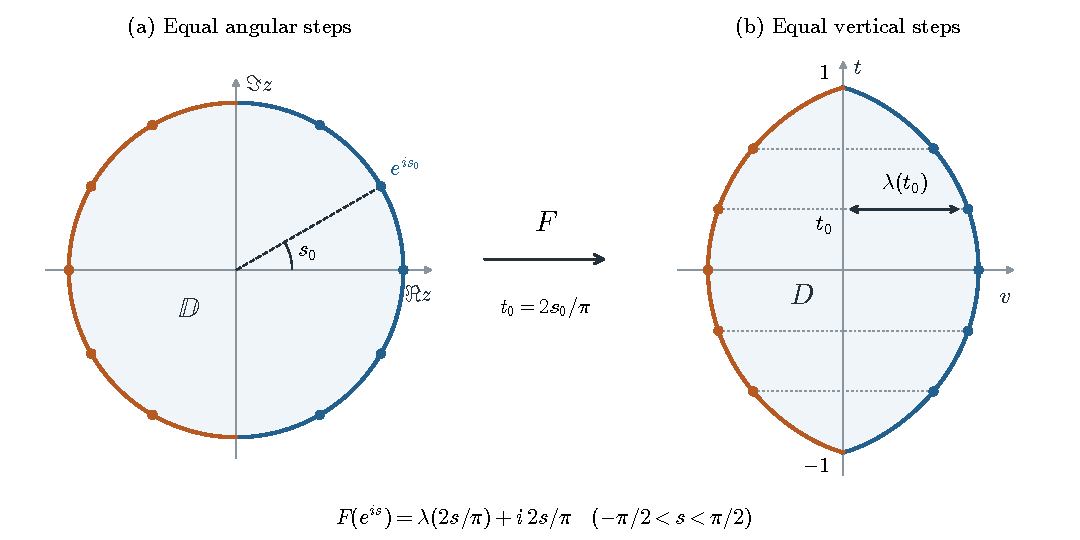
\includegraphics[width=\textwidth]{figures/lens-boundary-law.pdf}
\caption{The conformal lens and its boundary coordinate. Equally spaced
angles on either semicircle give equally spaced imaginary coordinates
on the corresponding boundary branch. On the right semicircle,
$F(e^{is})=\lambda(2s/\pi)+2is/\pi$; reflection gives the left branch.
Thus a uniform angle gives a uniform coordinate in $[-1,1]$ and an
independent fair branch sign. The horizontal arrow marks the
half-width $\lambda(t_0)$, with $s_0=\pi/6$ and $t_0=1/3$.}
\label{fig:lens-boundary-law}
\end{figure}

The two boundary graphs are smooth away from $\pm i$ and have strictly
turning tangent directions by \eqref{eq:lens-width-curvature}. In
particular, a fixed tangent line direction occurs at only finitely many
parameters away from these two endpoints. The boundary has planar
Lebesgue measure zero, as is also immediate from its graph description.

\begin{lemma}[Endpoint scaling]\label{lem:lens-endpoint}
As $\eta\downarrow0$,
\begin{equation}\label{eq:lens-endpoint-asymptotic}
 \lambda(1-\eta)=\frac2\pi\eta\log\frac1\eta+O(\eta).
\end{equation}
For every $0<a\leq b<\infty$,
\begin{equation}\label{eq:lens-endpoint-ratio}
 \sup_{a\leq c\leq b}
 \left|\frac{\lambda(1-\delta c)}{\lambda(1-\delta)}-c\right|
 \longrightarrow0\qquad(\delta\downarrow0).
\end{equation}
\end{lemma}

\begin{proof}
Equation~\eqref{eq:lens-width-curvature} and
$\operatorname{arctanh}(\cos x)=\log\cot(x/2)$ give
\[
 \lambda(1-\eta)=\frac2\pi\int_0^\eta
                  \log\cot\frac{\pi s}{4}\,ds.
\]
Here $\log\cot(\pi s/4)=\log(1/s)+O(1)$ uniformly as $s\downarrow0$.
Integration proves \eqref{eq:lens-endpoint-asymptotic}.
Writing $L=\log(1/\delta)$, the same uniform remainder gives
\[
 \frac{\lambda(1-\delta c)}{\lambda(1-\delta)}
 =c\,\frac{L-\log c+O(1)}{L+O(1)}
 =c+O_{a,b}(L^{-1})
\]
uniformly for $a\leq c\leq b$, which proves
\eqref{eq:lens-endpoint-ratio}.
\end{proof}

\section{Mass at an isolated holomorphic zero}
\label{sec:holomorphic-mass}

The next estimate turns the order of a holomorphic zero into an integral
bound for its Jacobian minors. Its application will use high powers of the
inverse planar map. In complex dimension $d$, the mass bound grows as the
$d$th power of their exponent, matching the radial rescaling that will produce boundary
feasibility probabilities in Section~\ref{sec:feasibility}.
The estimate is a special case of the sublevel-mass and comparison
formulas for generalized Lelong numbers; see
Demailly~\cite[Sections~3 and~5]{Demailly}. We give a direct Stokes
proof in the normalization used here.

On $\mathbb C^d$, write $z_j=x_j+iy_j$ and use the complex orientation
\[
dV=dx_1\wedge dy_1\wedge\cdots\wedge dx_d\wedge dy_d.
\]
For a smooth real function $v$, our convention is
\begin{equation}\label{eq:mass-dc-convention}
d^c=\frac{i}{4}(\bar\partial-\partial),
\qquad dd^c=\frac{i}{2}\partial\bar\partial.
\end{equation}
Thus $d^cv(\xi)=-\tfrac14dv(i\xi)$ for a real tangent vector $\xi$, and
\begin{equation}\label{eq:mass-volume-normalization}
dd^c|z|^2=\sum_{j=1}^d dx_j\wedge dy_j,
\qquad
(dd^cv)^d=d!\det(v_{\bar z_i z_j})\,dV.
\end{equation}
The second identity follows by expanding the exterior product, or by a
unitary diagonalization of the Hermitian Hessian.

\Needspace{8\baselineskip}
\begin{lemma}[Holomorphic mass]\label{lem:holomorphic-mass}
Let $d\geq1$, $N\geq d$, and let $\mathcal U\subset\mathbb C^d$ be open
and contain $0$. Suppose that $f=(f_1,\ldots,f_N):\mathcal U\to\mathbb C^N$
is holomorphic and has the following properties:
\begin{enumerate}
\item $f^{-1}(0)=\{0\}$;
\item for an integer $k\geq1$,
\[
f(z)=H(z)+O(|z|^{k+1})\quad\text{near }0,
\]
where each component of $H$ is a homogeneous polynomial of degree $k$
and $H(z)\ne0$ whenever $z\ne0$;
\item for every $0<s<1$, the set
$\{z\in\mathcal U:|f(z)|^2\leq s\}$ is compact in $\mathcal U$.
\end{enumerate}
Then, with $\tau=|f|^2$,
\begin{equation}\label{eq:holomorphic-minor-mass}
\int_{\{\tau<1\}}
 \sum_{\substack{I\subset\{1,\ldots,N\}\\|I|=d}}
 \left|\det\left(\frac{\partial f_i}{\partial z_j}\right)_{
                       i\in I,\ 1\leq j\leq d}\right|^2\,dV
\geq \frac{(\pi k)^d}{d!}.
\end{equation}
All norms are Euclidean. Rows in each determinant are in increasing index
order.
\end{lemma}

\begin{proof}
We first bound the integral of $(dd^c\tau)^d$. The conversion to
Jacobian minors will then follow from Cauchy--Binet.
Both $\tau$ and $\log\tau$ away from $0$ have positive semidefinite
complex Hessians. Indeed, if $Z$ is the complex derivative matrix of $f$,
the Hessian of $\tau$ is $Z^*Z$. For a complex direction $\xi$, the
Hessian of $\log\tau$ evaluates to
\[
\frac{|f|^2|df(\xi)|^2
       -|\langle df(\xi),f\rangle|^2}{|f|^4}\geq0
\]
by Cauchy--Schwarz. Their top exterior powers are therefore nonnegative.

\paragraph{Comparison with a small sphere.}
Fix a regular value $s\in(0,1)$ of $\tau$ and set
$E_s=\{z\in\mathcal U:\tau(z)<s\}$. By compactness of the sublevel and
the regular-value theorem, $\overline{E_s}$ is a compact smooth manifold
with boundary $\{\tau=s\}$. Stokes' theorem gives
\[
\int_{E_s}(dd^c\tau)^d
 =\int_{\partial E_s}d^c\tau\wedge(dd^c\tau)^{d-1}.
\]
Put $\gamma=d^c\log\tau$ on $\mathcal U\setminus\{0\}$. The identities
\[
d^c\log\tau=\tau^{-1}d^c\tau,
\qquad
dd^c\log\tau=\tau^{-1}dd^c\tau
                 -\tau^{-2}d\tau\wedge d^c\tau
\]
and the vanishing of the pullback of $d\tau$ to $\partial E_s$ imply
\begin{equation}\label{eq:mass-level-flux}
s^{-d}\int_{E_s}(dd^c\tau)^d
 =\int_{\partial E_s}\gamma\wedge(d\gamma)^{d-1}.
\end{equation}

For sufficiently small $\varepsilon>0$, the closed Euclidean ball
$\overline{B_\varepsilon}$ is contained in $E_s$. Orient
$S_\varepsilon=\partial B_\varepsilon$ outward from this ball. Applying
Stokes on $E_s\setminus\overline{B_\varepsilon}$ gives
\begin{equation}\label{eq:mass-punctured-flux}
s^{-d}\int_{E_s}(dd^c\tau)^d
 -\int_{S_\varepsilon}\gamma\wedge(d\gamma)^{d-1}
 =\int_{E_s\setminus\overline{B_\varepsilon}}
                     (dd^c\log\tau)^d\geq0.
\end{equation}
Thus it remains to determine the flux through a shrinking sphere.

\paragraph{The homogeneous flux.}
Let $T(z)=|H(z)|^2$ and $S=\{z:|z|=1\}$. The holomorphic Taylor
expansion implies
\[
\varepsilon^{-2k}\tau(\varepsilon z)\longrightarrow T(z)
\quad\text{in }C^2\text{ on a fixed closed annulus containing }S.
\]
For example, termwise differentiation of the convergent Taylor series
gives this convergence for the rescaled map and then for its squared
norm. Since $T$ is strictly positive on that annulus, the logarithms
converge in $C^2$ as well. Pulling back to $S$ by dilation, the additive
constant $2k\log\varepsilon$ disappears under $d^c$. Consequently
\begin{equation}\label{eq:mass-homogeneous-limit}
\lim_{\varepsilon\downarrow0}
 \int_{S_\varepsilon}\gamma\wedge(d\gamma)^{d-1}
 =\int_S\alpha\wedge(d\alpha)^{d-1},
\qquad \alpha=d^c\log T\big|_S.
\end{equation}

We compare this flux with that of the radial function $|z|^{2k}$.
Homogeneity gives
\[
T(rz)=r^{2k}T(z)\quad(r>0),\qquad T(e^{i\theta}z)=T(z).
\]
Thus $\log T-k\log|z|^2$ is unchanged by dilation and by common phase
rotation. These invariances will make its contribution to the flux
vanish. On $S$, put
\[
\alpha_0=d^c\log|z|^2\big|_S,
\qquad
\beta=d^c\bigl(\log T-k\log|z|^2\bigr)\big|_S,
\qquad
\alpha_t=k\alpha_0+t\beta\quad(0\leq t\leq1).
\]
Thus $\alpha_1=\alpha$.
For the nowhere-zero tangent vector field $V(z)=iz$ on $S$, the dilation
identity and \eqref{eq:mass-dc-convention} give
$\beta(V)=0$ and $\alpha_0(V)=1/2$. The phase-rotation identity makes every
$\alpha_t$ invariant under the flow of $V$. Cartan's identity therefore
gives
\[
\iota_Vd\alpha_t
 =\mathcal L_V\alpha_t-d\bigl(\alpha_t(V)\bigr)=0,
\]
where $\iota_V$ denotes contraction and $\mathcal L_V$ the Lie derivative.
It follows that the top-degree form
$\beta\wedge(d\alpha_t)^{d-1}$ on the $(2d-1)$-dimensional sphere
vanishes: its contraction with the nonzero vector $V$ is zero.
Differentiation and integration by parts on the closed sphere now yield
\[
\frac{d}{dt}\int_S\alpha_t\wedge(d\alpha_t)^{d-1}
 =d\int_S\beta\wedge(d\alpha_t)^{d-1}=0.
\]
For $d=1$ this is simply the derivative of $\int_S\alpha_t$; the same
argument applies.

On the unit sphere, $\alpha_0$ and $d\alpha_0$ are the restrictions of
$d^c|z|^2$ and $dd^c|z|^2$, respectively. Hence a final use of Stokes and
\eqref{eq:mass-volume-normalization} gives
\begin{align*}
\int_S\alpha\wedge(d\alpha)^{d-1}
 &=k^d\int_S\alpha_0\wedge(d\alpha_0)^{d-1}\\
 &=k^d\int_{\{|z|<1\}}(dd^c|z|^2)^d\\
 &=k^d d!\,\operatorname{vol}_{2d}(\{|z|<1\})
  =(\pi k)^d.
\end{align*}

\paragraph{The minor bound.}
Equations~\eqref{eq:mass-punctured-flux} and
\eqref{eq:mass-homogeneous-limit} imply
\[
\int_{E_s}(dd^c\tau)^d\geq s^d(\pi k)^d
\]
for every regular $s\in(0,1)$. Sard's theorem supplies an increasing
sequence of such values tending to $1$. Since the integrand is
nonnegative, monotone convergence gives
\[
\int_{\{\tau<1\}}(dd^c\tau)^d\geq(\pi k)^d.
\]
Finally, the complex Hessian $Z^*Z$ and Cauchy--Binet give the identity
\[
(dd^c\tau)^d
 =d!\sum_{|I|=d}|\det Z_I|^2\,dV.
\]
Division by $d!$ proves \eqref{eq:holomorphic-minor-mass}.
\end{proof}

\section{Feasible bases}\label{sec:feasibility}

We now apply the holomorphic mass estimate to finitely many real strip
constraints. It gives a lower bound for the sum of their boundary
feasibility probabilities. For the lens of Lemma~\ref{lem:planar-lens},
these probabilities will become volumes of real simplices.

Fix $d\geq1$ and nonzero real row vectors $b_1,\ldots,b_m$ spanning
$(\R^d)^*$. Write
\begin{equation}\label{eq:strip-body}
 A=\{X\in\R^d:|b_iX|\leq1\text{ for every }i\},
 \qquad C=A^\circ=\operatorname{conv}\{\pm b_1,\ldots,\pm b_m\}.
\end{equation}
We identify rows with vectors when taking a convex hull, and extend their
action complex-linearly to $\C^d$. The spanning assumption makes $A$
bounded, and $0\in\operatorname{int}A$. The polar identity follows from
the bipolar theorem: the polar of the displayed convex hull is exactly
$A$.
Let $\mathcal B$ be the collection of $d$-element sets of independent rows.
For $I\in\mathcal B$, put $B_I=(b_i)_{i\in I}$ in increasing index order
and $D_I=|\det B_I|$. Dependent row sets are omitted throughout.

For the next lemma, $F$ may be any biholomorphism of the unit disk onto a
bounded planar domain $D$, with $F(0)=0$ and a continuous extension to the
closed disk. For independent uniform angles $\theta_i\in[0,2\pi)$,
$i\in I$, define
\begin{equation}\label{eq:feasible-probabilities}
 Z_I(\theta)=B_I^{-1}\bigl(F(e^{i\theta_i})\bigr)_{i\in I},
 \qquad
 P_I=\mathbb P\{b_jZ_I(\theta)\in\overline D\text{ for all }j\},
 \qquad S=\sum_{I\in\mathcal B}P_I.
\end{equation}
The active coordinates $i\in I$ already belong to $\overline D$; thus the
probability tests only the remaining rows.

\begin{lemma}[Boundary feasibility]\label{lem:holomorphic-feasibility}
Let $d\ge1$ and let $b_1,\ldots,b_m$ be nonzero real rows spanning
$(\R^d)^*$. Let $F:\mathbb D\to D$ be a biholomorphism onto a bounded
planar domain, continuous on $\overline{\mathbb D}$, with $F(0)=0$.
Then the sum $S$ in \eqref{eq:feasible-probabilities} satisfies $S\ge1$.
No condition on extra-row boundary equalities or on dependent row
subsets is required.
\end{lemma}

\begin{proof}
Let $g=F^{-1}$ and set
\[
 \Omega=\{z\in\C^d:b_jz\in D\text{ for every }j\},
 \qquad h_j(z)=g(b_jz).
\]
The set $\Omega$ is open, bounded, and contains $0$. For an integer
$k\geq1$, apply Lemma~\ref{lem:holomorphic-mass} to the holomorphic map
\[
 f_k=(h_1^k,\ldots,h_m^k),\qquad
 \tau_k=\sum_{j=1}^m|h_j|^{2k}.
\]
We shall let $k$ tend to infinity. The mass lower bound has scale
$k^d$. The radial substitution below removes the same factor from the
Jacobian integrals and leaves a fixed domain on which the inferred
points tend to boundary samples.
The unique zero of $f_k$ is $0$: $g$ vanishes only at $0$, and the rows span.
Writing $c=g'(0)\ne0$, its degree-$k$ leading term is
$((cb_1z)^k,\ldots,(cb_mz)^k)$, also nonzero whenever $z\ne0$.
For $0<s<1$, the set $\{\tau_k\leq s\}$ is compact in $\Omega$.
Indeed each of its row coordinates belongs to the fixed compact set
$F(\{|w|\leq s^{1/(2k)}\})\subset D$. A basis of rows bounds $z$;
limits retain all these inclusions and the inequality $\tau_k\leq s$.
All hypotheses of the mass lemma therefore hold.
The derivative row of $h_j^k$ is a scalar multiple of $b_j$, so dependent
row subsets have zero minors. Consequently
\begin{equation}\label{eq:feasibility-mass}
 \sum_{I\in\mathcal B}M_{I,k}\geq
 k^d\frac{\pi^d}{d!},\qquad
 M_{I,k}:=\int_{\{\tau_k<1\}}
 \left|\det\frac{\partial(h_i^k)_{i\in I}}
                        {\partial(z_1,\ldots,z_d)}\right|^2\,dV_{2d}(z).
\end{equation}

Fix $I$. The change of variables $u_i=h_i(z)$, $i\in I$, is one-to-one
onto its image, with inverse
$z=B_I^{-1}(F(u_i))_{i\in I}$. Its squared complex Jacobian is its real
volume Jacobian. The squared determinant in $M_{I,k}$ is this Jacobian factor
times $k^{2d}\prod_i|u_i|^{2k-2}$.
The transformed integration domain is contained in
\[
 \left\{u\in\mathbb D^d:
       \sum_{i\in I}|u_i|^{2k}<1,\quad
       b_jB_I^{-1}(F(u_i))_{i\in I}\in D\text{ for all }j\right\}.
\]
We use this larger domain for an upper bound, and then put
$u_i=\rho_i^{1/k}e^{i\theta_i}$. The coordinate hyperplanes, on which
polar coordinates are undefined, have Lebesgue measure zero. Since
\[
 k^2|u_i|^{2k-2}\,dV_2(u_i)
      =k\rho_i\,d\rho_i\,d\theta_i,
\]
we obtain
\begin{equation}\label{eq:feasibility-radial}
 \frac{M_{I,k}}{k^d}\leq
 \int_{\substack{\rho_i>0,\ \sum_i\rho_i^2<1\\
                  \theta\in[0,2\pi)^d}}
 \mathbf1\!\left\{
  b_jB_I^{-1}\bigl(F(\rho_i^{1/k}e^{i\theta_i})\bigr)_{i\in I}
                    \in D\text{ for every }j\right\}
 \prod_{i\in I}\rho_i\,d\rho_i\,d\theta_i.
\end{equation}

The measure in this integral is finite: its total mass is the volume
$\pi^d/d!$ of the unit ball in $\C^d$. For every positive $\rho_i$,
continuity of $F$ on the closed disk makes the inferred points converge
to $Z_I(\theta)$. If a limiting row coordinate lies outside
$\overline D$, that constraint fails for all sufficiently large $k$.
Thus the upper limit of the indicator is bounded by the indicator of
the event defining $P_I$, including all possible boundary equalities.
The upper-bound form of Fatou's lemma, applied to functions bounded by
$1$ on this finite measure space, gives
\[
 \limsup_{k\to\infty}\frac{M_{I,k}}{k^d}
 \leq \frac{\pi^d}{d!}P_I.
\]
There are only finitely many bases, so \eqref{eq:feasibility-mass}
and these upper bounds give
\begin{align*}
 \frac{\pi^d}{d!}
 &\leq\limsup_{k\to\infty}
          \sum_{I\in\mathcal B}\frac{M_{I,k}}{k^d}\\
 &\leq\sum_{I\in\mathcal B}
          \limsup_{k\to\infty}\frac{M_{I,k}}{k^d}\\
 &\leq\frac{\pi^d}{d!}\sum_{I\in\mathcal B}P_I.
\end{align*}
Thus $S\geq1$.
\end{proof}

\subsection{Boundary equalities for the lens}

The lower bound for $S$ allows additional boundary equalities. The real
volume identity in Section~\ref{sec:simplex} will need the stronger fact
that these equalities have probability zero.
From now on, $F,D$, and $\lambda$ are those of
Lemma~\ref{lem:planar-lens}. We may also require that no two rows are
proportional. For any finite strip presentation this is achieved without
changing $A$ by keeping, on each row line, a row of largest magnitude;
its strip implies all the discarded strips on that line. Zero rows, if
present initially, impose no constraint and are discarded.
In dimension one the reduced list has a single row, so there are no
extra-row boundary equalities to consider.

\begin{lemma}[Additional boundary equalities have probability zero]
\label{lem:boundary-ties}
Let $F:\mathbb D\to D$ be the lens map of Lemma~\ref{lem:planar-lens}.
Assume that the nonzero spanning rows $b_1,\ldots,b_m$ are pairwise
nonproportional. For every $I\in\mathcal B$ and $j\notin I$,
\[
 \mathbb P\{b_jZ_I(\theta)\in\partial D\}=0.
\]
\end{lemma}

\begin{proof}
Write $b_jB_I^{-1}=(c_i)_{i\in I}$. At least two coefficients, say
$c_a,c_b$, are nonzero; otherwise $b_j$ would be proportional to a basis
row. Let $\gamma(\theta)=F(e^{i\theta})$.
Apart from its two endpoints, the lens boundary consists of the smooth
regular branches $(\pm\lambda(t),t)$, $-1<t<1$.
Their tangent directions have at most one occurrence on each branch for
any fixed unoriented line direction, because $\lambda'$ is strictly
monotone. The boundary parameter has constant nonzero speed in $t$ on
each branch, as established in the proof of Lemma~\ref{lem:planar-lens}.

Hold all phases other than $\theta_a,\theta_b$ fixed. The map
\[
 (\theta_a,\theta_b)\longmapsto
   c_a\gamma(\theta_a)+c_b\gamma(\theta_b)
       +\sum_{i\ne a,b}c_i\gamma(\theta_i)
\]
has real Jacobian determinant
$\det(c_a\gamma'(\theta_a),c_b\gamma'(\theta_b))$.
For every nonendpoint $\theta_a$, it vanishes at only finitely many
nonendpoint values of $\theta_b$. Its zero set, including the excluded
endpoint lines, therefore has planar measure zero by Fubini's theorem.
Off that set the inverse function theorem gives local diffeomorphism
charts. A countable subcover of such charts suffices, and in each chart
the inverse is locally Lipschitz, so it sends a planar null set to a null
set. The set $\partial D$ is planar-null, being a countable union of
compact smooth subarcs and two points. Its inverse image consequently
has measure zero in the two remaining phases. A final application of
Fubini over the fixed phases proves the assertion.
\end{proof}

\section{The real simplex identity}\label{sec:simplex}

The lens boundary law now turns the feasibility sum into an exact
integral over the strip body. The simplices in this integral lie in the
polar body; their missing volume will also be the quantity used in the
equality argument.

Keep the nonzero spanning, pairwise nonproportional rows of
\eqref{eq:strip-body}. For $X\in\operatorname{int}A$, define
\begin{equation}\label{eq:real-feasibility-body}
 L_X=\{Y\in\R^d:|b_jY|\leq\lambda(b_jX)
                         \text{ for every }j\}.
\end{equation}
All widths are strictly positive, so $L_X$ contains a neighborhood of
$0$; a basis of rows shows that it is bounded. It is therefore a convex
polytope with nonempty interior.
For a basis $I$ and signs $\epsilon=(\epsilon_i)_{i\in I}\in\{-1,1\}^I$,
let
\[
 Y_{I,\epsilon}(X)=B_I^{-1}
          \bigl(\epsilon_i\lambda(b_iX)\bigr)_{i\in I}.
\]
We call $(I,\epsilon)$ feasible at $X$ when this vector belongs to $L_X$.
This definition specifies a unique vector for every choice, whether or
not it is feasible. Set
\begin{equation}\label{eq:feasible-simplex-union}
 T_{I,\epsilon}=\operatorname{conv}
                  \bigl(0,\{\epsilon_i b_i:i\in I\}\bigr),
 \qquad
 \Sigma_X=\bigcup_{(I,\epsilon)\text{ feasible at }X}T_{I,\epsilon}.
\end{equation}
Thus $\Sigma_X$ is a finite union of closed $d$-simplices contained in
$C=A^\circ$. This definition applies at every interior $X$, including
points with additional tight constraints. For integration only, declare
every pair infeasible and set $\Sigma_X=\varnothing$ when
$X\in\partial A$.

A feasible pair specifies a vertex $Y_{I,\epsilon}(X)$ of $L_X$.
A strictly positive combination of its signed tight rows defines a
linear functional maximized uniquely at that vertex. This is why
different feasible pairs give simplices with disjoint interiors
whenever their vertices are distinct. The proof below removes, outside
a null set of $X$, the boundary ties that could make two pairs specify
the same vertex.

\begin{proposition}[Feasible-simplex identity]\label{prop:simplex-integral}
Let $b_1,\ldots,b_m$ be nonzero, pairwise nonproportional real rows
spanning $(\R^d)^*$, and let $F,D,\lambda$ be as in
Lemma~\ref{lem:planar-lens}. With $A$, $S$, and $\Sigma_X$ defined in
\eqref{eq:strip-body}, \eqref{eq:feasible-probabilities}, and
\eqref{eq:feasible-simplex-union}, respectively,
\begin{equation}\label{eq:simplex-integral}
 1\leq S
   =\frac{d!}{4^d}\int_A|\Sigma_X|\,dX
   \leq\frac{d!}{4^d}|A|\,|A^\circ|.
\end{equation}
In particular, $|A|\,|A^\circ|\geq4^d/d!$, and
\begin{equation}\label{eq:simplex-deficit}
 0\leq\int_A\bigl(|A^\circ|-|\Sigma_X|\bigr)\,dX
       \leq |A|\,|A^\circ|-\frac{4^d}{d!}.
\end{equation}
\end{proposition}

\begin{proof}
We first convert each probability into a real integral. By
\eqref{eq:lens-boundary-law}, each active boundary coordinate has the
law $\epsilon_i\lambda(t_i)+it_i$, with $t_i$ uniform on $[-1,1]$ and
$\epsilon_i$ an independent fair sign. Consequently each fixed sign
choice has joint measure $4^{-d}\,dt_I$ on $[-1,1]^d$.
Writing the inferred complex vector as $Y+iX$ gives
\[
 t_I=B_IX,\qquad Y=Y_{I,\epsilon}(X).
\]
The constraints that all row coordinates lie in $\overline D$ are
exactly $X\in A$ and $Y\in L_X$, apart from the immaterial boundary
$\partial A$. This boundary has measure zero, since it is contained in
the finitely many hyperplanes $b_jX=\pm1$. The change of variables
$t_I=B_IX$ therefore gives
\begin{equation}\label{eq:probability-real-integral}
 P_I=\frac{D_I}{4^d}\int_A
       \sum_{\epsilon\in\{-1,1\}^I}
         \mathbf1\{(I,\epsilon)\text{ is feasible at }X\}\,dX.
\end{equation}

For almost every $X\in\operatorname{int}A$, every feasible pair
$(I,\epsilon)$ has no tight constraint outside $I$. Indeed, such an
additional equality means that an extra row of $Y+iX$ lies on
$\partial D$. Lemma~\ref{lem:boundary-ties} makes this event null in the
basis phases; the boundary law and the invertible change $t_I=B_IX$
make its set of $X$ null for each fixed sign choice. There are finitely
many bases, sign choices, and extra rows, so a single null set removes
all these equalities.

Fix $X$ outside this null set. Distinct feasible pairs have distinct
vectors $Y_{I,\epsilon}(X)$. If their bases differ, a shared vector would
have a tight row outside one of the bases. If their bases agree but
some signs differ, the shared vector would satisfy opposite equations
with the same strictly positive width, which is impossible.

The interiors of their simplices are disjoint. To see this, let
$e\in\operatorname{int}T_{I,\epsilon}$. It has a representation
$e=\sum_{i\in I}\alpha_i\epsilon_i b_i$ with all $\alpha_i>0$ and
$\sum_i\alpha_i<1$. For every $Y\in L_X$,
\[
 eY\leq\sum_{i\in I}\alpha_i\lambda(b_iX),
\]
and equality holds at $Y_{I,\epsilon}(X)$. Equality forces every
independent equation
$\epsilon_i b_iY=\lambda(b_iX)$, so this is the unique maximizer of the
linear functional $e$ on $L_X$. If $e$ belonged to the interiors of two
feasible simplices, their distinct vectors would both be its unique
maximizer, a contradiction.
Each simplex has volume $D_I/d!$, and their boundaries have measure
zero. It follows that, for almost every $X$,
\begin{equation}\label{eq:simplex-volume-sum}
 d!\,|\Sigma_X|
      =\sum_{I\in\mathcal B}\sum_{\epsilon\in\{-1,1\}^I}
               D_I\,\mathbf1\{(I,\epsilon)\text{ is feasible at }X\}.
\end{equation}

All integrals here are measurable. For each pair, feasibility is a
finite collection of closed inequalities between continuous functions
of $X\in\operatorname{int}A$. In particular the set
\[
 \{(X,e):X\in\operatorname{int}A,\ e\in\Sigma_X\}
\]
is a finite union of products of Borel feasibility sets and fixed
closed simplices. Fubini's theorem makes $X\mapsto|\Sigma_X|$
measurable, and it is bounded by $|C|$.
Sum \eqref{eq:probability-real-integral}, use
\eqref{eq:simplex-volume-sum}, and apply
Lemma~\ref{lem:holomorphic-feasibility}. This proves the first equality
and lower bound in \eqref{eq:simplex-integral}. The containment
$\Sigma_X\subset C$ proves the upper bound. In particular, the missing
volume has the exact expression
\[
 \int_A\bigl(|C|-|\Sigma_X|\bigr)\,dX
   =|A|\,|C|-\frac{4^d}{d!}S.
\]
It is nonnegative by containment, and $S\geq1$ bounds it above by
$|A|\,|C|-4^d/d!$. This proves \eqref{eq:simplex-deficit} and identifies
the quantity that will tend to zero in the equality argument.
\end{proof}

For a concrete union with positive missing volume, take
$b_1=(1,0)$, $b_2=(1/2,\sqrt3/2)$, $b_3=b_2-b_1$, and
$X=0.9(1,1/\sqrt3)$, as in Figure~\ref{fig:feasible-simplex-deficit}.
Then $b_1X=b_2X=0.9$ and $b_3X=0$. Write $a=\lambda(0.9)$.
The endpoint
integral for $\lambda$ and $\cot x<1/x$ for $0<x<\pi/2$ give
\[
 a<\frac{\log(40/\pi)+1}{5\pi}<\frac4{15},
 \qquad
 \lambda(0)>\frac8{\pi^2}\left(1-\frac19\right)
             >\frac{32}{45}.
\]
The second bound uses the alternating series for $F(1)$. In particular,
$2a<\lambda(0)$, so the third strip in the example is strictly redundant.

\begin{figure}[htbp]
\centering
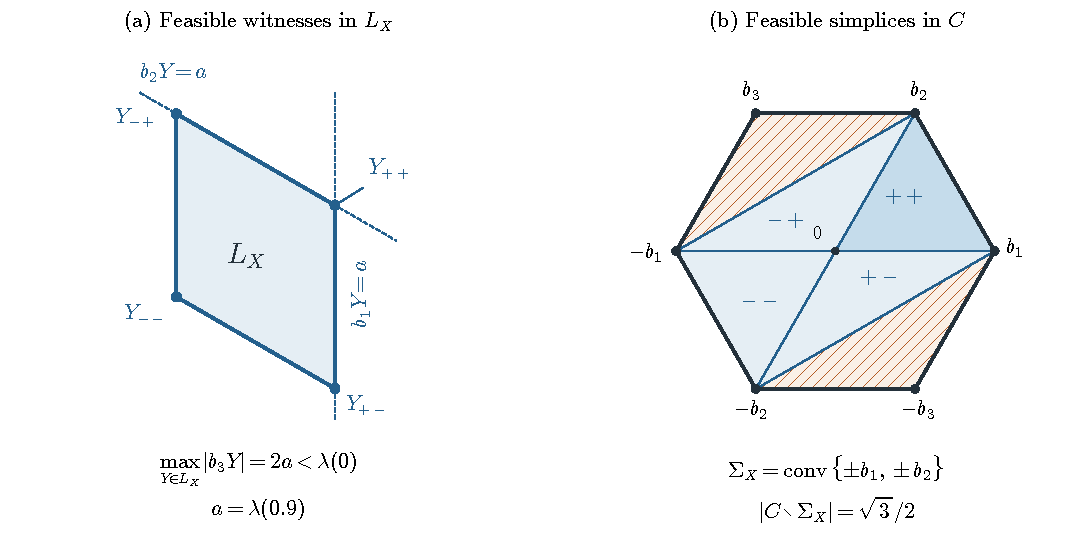
\includegraphics[width=\textwidth]{figures/feasible-simplex-deficit.pdf}
\caption{A feasible-simplex union can leave part of the polar uncovered.
Here $b_1=(1,0)$, $b_2=(1/2,\sqrt3/2)$,
$b_3=(-1/2,\sqrt3/2)$, $C=\operatorname{conv}\{\pm b_1,\pm b_2,\pm b_3\}$,
and $X=0.9(1,1/\sqrt3)$.
The third strip is redundant in $L_X$, as verified above. The four witnesses
$Y_{\epsilon_1\epsilon_2}$, defined by
$b_iY=\epsilon_i a$ for $i=1,2$, correspond to the four triangles
$\operatorname{conv}(0,\epsilon_1b_1,\epsilon_2b_2)$ with matching sign
labels. Their union is $\Sigma_X=\operatorname{conv}\{\pm b_1,\pm b_2\}$.
The two hatched caps have total area $\sqrt3/2$, one third of $|C|$.}
\label{fig:feasible-simplex-deficit}
\end{figure}

\subsection{Approximation of an arbitrary convex body}

\begin{corollary}[The symmetric volume-product inequality]
\label{cor:symmetric-inequality}
For every origin-symmetric convex body $K\subset\R^d$, $d\geq1$,
\[
 |K|\,|K^\circ|\geq\frac{4^d}{d!}.
\]
\end{corollary}

\begin{proof}
Put $Q=K^\circ$ and choose $a>0$ with $aB_2^d\subset Q$,
where $B_2^d$ is the Euclidean unit ball.
For $\varepsilon_j\downarrow0$, take a finite $\varepsilon_j$-net in
$Q$, adjoin its negatives, and let $Q_j$ be its convex hull. Thus
$Q_j\subset Q$, and their support functions satisfy, for every Euclidean
unit vector $u$,
\[
 h_Q(u)-\varepsilon_j\leq h_{Q_j}(u)\leq h_Q(u),
 \qquad h_Q(u)\geq a.
\]
For $\delta_j=\varepsilon_j/a<1$, this implies
\begin{equation}\label{eq:polar-approximation}
 (1-\delta_j)Q\subset Q_j\subset Q,
 \qquad
 K\subset A_j:=Q_j^\circ\subset(1-\delta_j)^{-1}K.
\end{equation}
The first inclusions follow from the support-function inequalities and
convex separation; the second follow by polarity. In particular $Q_j$
and $A_j$ are full-dimensional symmetric polytopes for large $j$.

Choose one vertex from each antipodal vertex pair of $Q_j$ as a row
list. These rows are nonzero and span. They are pairwise
nonproportional: two distinct boundary vertices on the same ray from
an interior origin cannot both be extreme, and the antipodal duplication
has already been removed. Their strip body is $A_j$.
Proposition~\ref{prop:simplex-integral} therefore gives
$|A_j|\,|Q_j|\geq4^d/d!$.
The homothetic bounds \eqref{eq:polar-approximation} show both
$|Q_j|\to|Q|$ and $|A_j|\to|K|$, because dilation by $t>0$ multiplies
volume by $t^d$. Passing to the limit proves the assertion. No smoothness,
simplicity, or general-position assumption is imposed on $K$.
In dimension one the assertion can also be read directly:
$K=[-a,a]$ has polar $[-1/a,1/a]$ and product $4$.
\end{proof}

\section{Equality and a common feasibility witness}
\label{sec:zero-deficit}

The integral in \eqref{eq:simplex-integral} measures how much of the
polar body is covered by feasible simplices. For a body attaining the
sharp volume product, we shall make the uncovered volume tend to zero
after adjoining one segment. Compactness then gives a feasible witness
at every interior point and in every direction. The resulting
representation will be the input to the equality classification.

Throughout this section $K=-K\subset\mathbb R^n$ is a convex body,
$n\ge1$, satisfying
\[
 |K|\,|K^\circ|=\frac{4^n}{n!}.
\]
Set $Q=K^\circ$, $d=n+1$, and
\begin{equation}\label{eq:segment-lift}
 B=K\oplus_1[-1,1]
   =\{(x,s):p_K(x)+|s|\le1\},
 \qquad C=B^\circ=Q\times[-1,1].
\end{equation}
The polar $C$ has the two horizontal faces $Q\times\{1\}$ and
$Q\times\{-1\}$. The representations constructed below will use
vectors from these faces.
In this lifted space, $X$ and $Y$ belong to $\mathbb R^d$, while elements of $C$
act on them by the Euclidean pairing. Recall that the lens width
$\lambda:[-1,1]\to[0,\infty)$ is continuous, even and concave, with
$\lambda(0)>0$ and $\lambda(t)\le\lambda(0)$.

\begin{proposition}[A representation minimizing the lens cost]
\label{prop:optimal-representation}
Let $K\subset\mathbb R^n$, $n\ge1$, be an origin-symmetric convex body
with $P(K)=4^n/n!$. Put $Q=K^\circ$, $d=n+1$, and define the lifted
bodies $B,C$ by \eqref{eq:segment-lift}.
For every $X\in\operatorname{int}B$ and every nonzero
$\xi=(q,a)\in\mathbb R^n\times\mathbb R$, put
\[
 T=p_C(\xi)=\max\{p_Q(q),|a|\}.
\]
There are $1\le r\le d$ vectors $c_i=(b_i,\sigma_i)$ with
$b_i\in Q$ and $\sigma_i\in\{-1,1\}$, nonnegative numbers
$\alpha_i$, and a vector $Y\in\mathbb R^d$, such that
\begin{equation}\label{eq:optimal-representation}
 \xi=\sum_{i=1}^r\alpha_i c_i,
 \qquad \sum_{i=1}^r\alpha_i=T,
\end{equation}
and
\begin{equation}\label{eq:common-witness}
 |h\cdot Y|\le\lambda(h\cdot X)\quad(h\in C),
 \qquad
 c_i\cdot Y=\lambda(c_i\cdot X)\quad(1\le i\le r).
\end{equation}
In particular, for every finite representation
$\xi=\sum_{j=1}^s\beta_jh_j$ with $\beta_j\ge0$ and $h_j\in C$,
\begin{equation}\label{eq:optimal-cost}
 \sum_{i=1}^r\alpha_i\lambda(c_i\cdot X)
 \le \sum_{j=1}^s\beta_j\lambda(h_j\cdot X).
\end{equation}
The choices may depend on $X$ and $\xi$; the same choice satisfies
\eqref{eq:optimal-cost} for all the competing representations.
\end{proposition}

The last coordinates $\sigma_i$ split the chosen rows into two groups.
In Section~\ref{sec:median}, we compare representation costs as $X$ approaches
the apex $(0,1)$ of $B$; the endpoint behavior of $\lambda$ makes the
two signs contribute differently. We now prove
Proposition~\ref{prop:optimal-representation} in three steps: approximate
$C$ by polytopes, locate feasible simplices near each prescribed point
and direction, and pass to a common witness to compare costs.

\subsection{Inner polytopes and vanishing missing volume}

The horizontal section of $B$ at height $s\in[-1,1]$ is
$(1-|s|)K$. Hence
\[
 |B|=|K|\int_{-1}^1(1-|s|)^n\,ds
     =\frac{2|K|}{n+1},
 \qquad |C|=2|Q|,
\]
and therefore
\begin{equation}\label{eq:lift-equality}
 |B|\,|C|=\frac4{n+1}|K|\,|Q|=\frac{4^d}{d!}.
\end{equation}

Choose full-dimensional symmetric polytopes $Q_j\subset Q$
converging to $Q$ in Hausdorff distance. For example, take the convex
hulls of increasingly fine finite symmetric nets in $Q$, including
a fixed spanning symmetric set. There are numbers $t_j\in(0,1)$
with $t_j\to1$ such that
\[
 t_jQ\subseteq Q_j\subseteq Q.
\]
Indeed, if $Q$ contains a Euclidean ball of radius $r_0>0$ and the
Hausdorff error is $\varepsilon_j$, then on Euclidean unit directions
\[
 h_{Q_j}\ge h_Q-\varepsilon_j
          \ge (1-\varepsilon_j/r_0)h_Q.
\]
The support-function criterion for containment gives the claim,
after discarding finitely many indices and choosing $t_j$ slightly
smaller if necessary.

Put $C_j=Q_j\times[-1,1]$ and $B_j=C_j^\circ$. The inclusions above
give
\begin{equation}\label{eq:lift-sandwich}
 t_jC\subseteq C_j\subseteq C,
 \qquad
 B\subseteq B_j\subseteq t_j^{-1}B.
\end{equation}
In particular, $|B_j|\,|C_j|\to|B|\,|C|$.
Use one row from each antipodal vertex pair of $C_j$ to describe $B_j$
as an intersection of strips. These rows span $\mathbb R^d$, and
no two are proportional: a ray from the interior point $0$ meets the
boundary of a convex body in only one point. Every signed row is a
vertex of $C_j$, and thus belongs to $Q_j\times\{-1,1\}$.

Let $\Sigma_{j,X}$ be the union of the feasible signed basis
simplices for this strip description, as in
\eqref{eq:simplex-integral}. In particular, for every
$X\in\operatorname{int}B_j$ it is a finite union of closed simplices
contained in $C_j$. Its definition is retained also at the exceptional
interior points where several constraints are simultaneously tight.
The integral estimate and \eqref{eq:lift-equality} imply
\begin{equation}\label{eq:vanishing-missing-volume}
 \begin{split}
 0\le D_j
 &:=\int_{B_j}\bigl(|C_j|-|\Sigma_{j,X}|\bigr)\,dX\\
 &\le |B_j|\,|C_j|-\frac{4^d}{d!}
 \longrightarrow0.
 \end{split}
\end{equation}

\subsection{From an integral deficit to each point and direction}

Fix $X\in\operatorname{int}B$ and $e\in\partial C$. We first
construct indices $j_k\to\infty$ and points
\begin{equation}\label{eq:nearby-feasible-pairs}
 X_k\in\operatorname{int}B_{j_k},\qquad
 e_k\in\Sigma_{j_k,X_k},\qquad
 (X_k,e_k)\longrightarrow(X,e).
\end{equation}
This is a consequence of \eqref{eq:vanishing-missing-volume} on
product neighborhoods; it does not require a pointwise limit of the
functions $X\mapsto|\Sigma_{j,X}|$.

For each $k$, choose a Euclidean ball $U_k$ of positive volume
contained in $\operatorname{int}B\cap B(X,1/k)$. There is also a ball
$V_k$ of positive volume with closure contained in
$\operatorname{int}C\cap B(e,1/k)$. To see this at the boundary point
$e$, first move a small distance from $e$ toward $0$; the resulting
point is interior because $0\in\operatorname{int}C$. Take a sufficiently
small ball about that point. By \eqref{eq:lift-sandwich},
$U_k\subset\operatorname{int}B_j$ for every $j$, and
$V_k\subset C_j$ for all sufficiently large $j$. The second assertion
follows also from $\max_{h\in\overline{V_k}}p_C(h)<1$ and $t_j\to1$.

Choose $j_k>j_{k-1}$ so large that these inclusions hold and
$D_{j_k}<|U_k|\,|V_k|$. If $\Sigma_{j_k,Z}$ missed $V_k$ for every
$Z\in U_k$, its missing volume would be at least $|V_k|$ throughout
$U_k$, contradicting this inequality. Thus choose
$X_k\in U_k$ and $e_k\in\Sigma_{j_k,X_k}\cap V_k$.
This proves \eqref{eq:nearby-feasible-pairs}.

Choose one feasible simplex containing $e_k$. Its $d$ signed basis
rows, written $c_{1k},\ldots,c_{dk}\in Q_{j_k}\times\{-1,1\}$,
give weights $\theta_{ik}\ge0$ satisfying
\begin{equation}\label{eq:approximate-representation}
 e_k=\sum_{i=1}^d\theta_{ik}c_{ik},
 \qquad \sum_{i=1}^d\theta_{ik}\le1.
\end{equation}
The coefficient left over is the weight of the simplex vertex $0$.
Feasibility supplies one vector $Y_k$ such that
\[
 c_{ik}\cdot Y_k=\lambda(c_{ik}\cdot X_k)\quad(1\le i\le d),
 \qquad
 |v\cdot Y_k|\le\lambda(v\cdot X_k)
 \quad\text{for every vertex $v$ of $C_{j_k}$}.
\]
Here a sign on a basis row has been absorbed using the evenness of
$\lambda$.

The last inequality extends to all $h\in C_{j_k}$. Indeed, write
$h=\sum_\ell s_\ell v_\ell$ as a convex combination of vertices.
The triangle inequality followed by concavity gives
\[
 |h\cdot Y_k|
 \le\sum_\ell s_\ell|v_\ell\cdot Y_k|
 \le\sum_\ell s_\ell\lambda(v_\ell\cdot X_k)
 \le\lambda(h\cdot X_k).
\]
Consequently $Y_k\in\lambda(0)B_{j_k}$. The polar sandwich
\eqref{eq:lift-sandwich} makes these witnesses uniformly bounded,
even if the selected bases approach singularity.

Pass to a subsequence on which $Y_k\to Y$, every $c_{ik}\to c_i$,
and every $\theta_{ik}\to\theta_i$. This uses a fixed finite product
of compact sets: all rows belong to $Q\times\{-1,1\}$ and all
weights belong to $[0,1]$. No independence of the limiting rows is
needed. We have
\[
 c_i\in Q\times\{-1,1\},\qquad
 e=\sum_{i=1}^d\theta_i c_i,\qquad
 \theta_i\ge0,\qquad \sum_i\theta_i\le1,
\]
and continuity of $\lambda$ gives
$c_i\cdot Y=\lambda(c_i\cdot X)$ for all $i$.
For arbitrary $h\in C$, use $h_k=t_{j_k}h\in C_{j_k}$ in the
feasibility inequality and pass to the limit. It follows that
\begin{equation}\label{eq:limiting-feasibility}
 |h\cdot Y|\le\lambda(h\cdot X)\qquad(h\in C).
\end{equation}
The subsequence has already been fixed; this argument proves
\eqref{eq:limiting-feasibility} for all $h$ with the same $Y$.

Since $e\in\partial C$, its gauge is one. Therefore
\[
 1=p_C(e)\le\sum_{i=1}^d\theta_i p_C(c_i)
   \le\sum_{i=1}^d\theta_i\le1.
\]
Thus $\sum_i\theta_i=1$: none of the limiting mass remains at the
simplex vertex $0$.

\subsection{Comparison with every positive representation}

To prove Proposition~\ref{prop:optimal-representation}, fix its
$X$ and nonzero $\xi$, and apply the preceding construction to
$e=\xi/T\in\partial C$. Set $\alpha_i=T\theta_i$ and discard any
zero weights if desired. This gives at most $d$ rows and proves
\eqref{eq:optimal-representation} and \eqref{eq:common-witness}.
For any finite competing representation
$\xi=\sum_j\beta_jh_j$, $\beta_j\ge0$, $h_j\in C$, the common
witness gives
\[
 \sum_i\alpha_i\lambda(c_i\cdot X)
 =\xi\cdot Y
 =\sum_j\beta_j h_j\cdot Y
 \le\sum_j\beta_j\lambda(h_j\cdot X).
\]
This proves \eqref{eq:optimal-cost} and completes the proof of
Proposition~\ref{prop:optimal-representation}. In particular,
the conclusion holds for each prescribed $X$ and $\xi$, including
directions for which every limiting representation is degenerate.

\section{From endpoint costs to metric medians}\label{sec:median}

We now convert the optimal representations into a geometric property
of the polar body. A \emph{metric median} of three points in a normed
space is a point that lies between every pair: if the points are
$x_0,x_1,x_2$, a median $m$ satisfies
\[
 \|x_i-x_j\|=\|x_i-m\|+\|m-x_j\|
 \qquad(0\le i<j\le2).
\]
The median need not be unique. Its existence will imply the ball
intersection property that characterizes linear Hanner bodies.

\begin{proposition}[Medians of an equality body]\label{prop:metric-median}
Let $K\subset\R^n$, $n\ge1$, be an origin-symmetric convex body with
$P(K)=4^n/n!$, and put $Q=K^\circ$. Every triple of points in
$(\R^n,p_Q)$ has a metric median.
\end{proposition}

\begin{proof}
Write $\|\cdot\|=p_Q$. Translation reduces the triple to $0,x,y$.
If two points coincide, that repeated point is a median, so assume
that $0,x,y$ are distinct. Set
\[
 p_1=\|x\|,\qquad p_2=\|y\|,\qquad p=\|x-y\|,
 \qquad s=p_1+p_2,\qquad a=p_1-p_2.
\]
All three distances are positive. The triangle and reverse triangle
inequalities give $s\ge p\ge|a|$. Define
\begin{equation}\label{eq:median-radii}
 A_+=\frac{p+a}{2},\qquad A_-=\frac{p-a}{2},
 \qquad c=\frac{s-p}{2}.
\end{equation}
These numbers are nonnegative, with
$A_++A_-=p$, $c+A_+=p_1$, and $c+A_-=p_2$.

\paragraph{The compact set of aggregate directions.}
Let
\begin{equation}\label{eq:aggregate-set}
 D_0=\{r_+-r_-:\ r_++r_-=x-y,\quad
                  \|r_+\|\le A_+,\quad\|r_-\|\le A_-\}.
\end{equation}
Our goal is to prove $x+y\in D_0+(s-p)Q$. Such membership supplies
$r_+,r_-$ for which $m=x-r_+=y+r_-$ has distances to $0,x,y$
bounded by $c,A_+,A_-$, respectively; the triangle inequalities then
force the three median equalities. We shall prove this membership by
estimating support functions in each direction.

The set $D_0$ is compact and convex: it is the linear image of the intersection
of $A_+Q\times A_-Q$ with the affine subspace $r_++r_-=x-y$. It is nonempty, since
$r_\pm=(A_\pm/p)(x-y)$ satisfy the constraints. This also covers
$A_+=0$ or $A_-=0$.

\paragraph{Endpoint comparison.}
Fix $u\in\operatorname{int}K$ and let
$X_\delta=(\delta u,1-\delta)$, $0<\delta<1$. The lifted body
$B=K\oplus_1[-1,1]$ contains $X_\delta$ in its interior because
\[
 p_B(X_\delta)=\delta p_K(u)+1-\delta<1.
\]
Apply Proposition~\ref{prop:optimal-representation} with this $X_\delta$
and $(q,a)=(x-y,p_1-p_2)$. Its total weight is
$T=\max\{\|q\|,|a|\}=p$. We obtain rows
$(b_i,\sigma_i)\in Q\times\{-1,1\}$ and weights $\alpha_i\ge0$
satisfying \eqref{eq:optimal-representation} and
\eqref{eq:optimal-cost}. Their aggregates
\[
 r_\pm=\sum_{\sigma_i=\pm1}\alpha_i b_i
\]
have $r_++r_-=x-y$. Since
$\sum_{\sigma_i=\pm1}\alpha_i=(p\pm a)/2=A_\pm$, they satisfy
$\|r_\pm\|\le A_\pm$ and hence $r_+-r_-\in D_0$.
No choice of these representations across different $u$ or $\delta$
is required.

For $b\in Q$ and $\sigma=\pm1$, evenness of $\lambda$ gives
\[
 \lambda\bigl(\langle(b,\sigma),X_\delta\rangle\bigr)
 =\lambda\bigl(1-\delta(1-\sigma\langle b,u\rangle)\bigr).
\]
The factors $1-\sigma\langle b,u\rangle$ belong to
$[1-p_K(u),1+p_K(u)]$, a compact subinterval of $(0,\infty)$.
Lemma~\ref{lem:lens-endpoint} therefore gives an error
$\varepsilon_u(\delta)\to0$ such that
\begin{equation}\label{eq:median-endpoint-error}
 \left|
 \frac{\lambda(\langle(b,\sigma),X_\delta\rangle)}
      {\lambda(1-\delta)}
       -1+\sigma\langle b,u\rangle
 \right|\le\varepsilon_u(\delta)
 \quad(b\in Q,\ \sigma=\pm1).
\end{equation}
In particular, the normalized cost of the optimal representation is
at least
\[
 p-\langle r_+-r_-,u\rangle-p\varepsilon_u(\delta)
 \ge p-h_{D_0}(u)-p\varepsilon_u(\delta).
\]
Compare this cost, using \eqref{eq:optimal-cost}, with the two-term
representation
\[
 (x-y,a)=p_1(x/p_1,1)+p_2(-y/p_2,-1).
\]
Both rows belong to $Q\times\{-1,1\}$. By
\eqref{eq:median-endpoint-error}, their normalized cost tends to
$s-\langle x+y,u\rangle$. Letting $\delta\downarrow0$ yields
\begin{equation}\label{eq:median-support-interior}
 \langle x+y,u\rangle\le h_{D_0}(u)+s-p
 \qquad(u\in\operatorname{int}K).
\end{equation}
The error was uniform only over $b,\sigma$ for the fixed $u$; that
is all this limit requires.

\paragraph{Separation and the median.}
Continuity extends \eqref{eq:median-support-interior} to $u\in K$.
For any nonzero $v\in\R^n$, the point
$u=v/h_Q(v)$ lies on $\partial K$, by \eqref{eq:gauge-support}.
Homogeneity of support functions gives
\[
 \langle x+y,v\rangle\le h_{D_0}(v)+(s-p)h_Q(v).
\]
The same inequality holds at $v=0$. The right side is the support
function of the compact convex set $D_0+(s-p)Q$, with the convention
$0Q=\{0\}$. Convex separation therefore implies
\begin{equation}\label{eq:median-membership}
 x+y\in D_0+(s-p)Q.
\end{equation}
Choose the corresponding pair $r_+,r_-$ in
\eqref{eq:aggregate-set}, and put
\[
 m=x-r_+=y+r_-.
\]
Then $2m=x+y-(r_+-r_-)$, so \eqref{eq:median-membership} gives
\[
 \|m\|\le c,\qquad
 \|x-m\|\le A_+,\qquad
 \|y-m\|\le A_-.
\]
The triangle inequality forces all three bounds to be equalities:
\[
 \begin{aligned}
 p_1&\le\|m\|+\|x-m\|\le c+A_+=p_1,\\
 p_2&\le\|m\|+\|y-m\|\le c+A_-=p_2.
 \end{aligned}
\]
Thus $m$ lies between $0,x$ and between $0,y$, and
\[
 \|x-m\|+\|m-y\|=A_++A_-=p=\|x-y\|.
\]
This proves the median property. The argument permits $c=0$ or either
$A_\pm=0$, so saturated triangle inequalities require no limiting
argument.
\end{proof}

\subsection{Three balls and the equality classification}

A normed space has the \emph{three-ball intersection property}, also
called the \emph{3.2 intersection property}, if any three closed balls
that intersect pairwise have a common point. Their radii may differ. The equivalence between this intersection
property and the metric-median condition is Lima's classical
norm-additive decomposition criterion~\cite[Theorem~1.2]{Lima1978};
see also Hansen--Lima~\cite[Theorem~3.6(4)]{HansenLima1981}. We include the
short direction needed here, with arbitrary radii.

\begin{lemma}[From medians to three balls]\label{lem:three-balls}
Suppose every triple of points in a real normed space has a metric
median. Then the space has the three-ball intersection property,
including balls of radius zero.
\end{lemma}

\begin{proof}
Consider pairwise-intersecting balls with centers $x_1,x_2,x_3$ and
radii $r_1,r_2,r_3\ge0$. Let $m$ be a metric median of their centers,
and set $d_i=\|m-x_i\|$. Pairwise intersection and the median property
imply
\[
 d_i+d_j=\|x_i-x_j\|\le r_i+r_j
 \qquad(i\ne j).
\]
If every $d_i\le r_i$, the median is a common point. Otherwise,
after relabeling, $t=d_1-r_1>0$. For $j=2,3$ the displayed inequalities
give $d_j+t\le r_j$, so no other ball excludes $m$. Since
$0<t\le d_1$, the point
\[
 z=m+\frac{t}{d_1}(x_1-m)
\]
is well defined and lies on the segment from $m$ to $x_1$. It satisfies
\[
 \begin{aligned}
 \|z-x_1\|&=d_1-t=r_1,\\
 \|z-x_j\|&\le\|z-m\|+d_j=t+d_j\le r_j\quad(j=2,3).
 \end{aligned}
\]
Thus $z$ lies in all three balls. This includes $r_1=0$, when $z=x_1$.
\end{proof}

The required structure theorem is due to Hansen and Lima. In their
terminology the balls are closed and have arbitrary radii
\cite[Section~1]{HansenLima1981}.

\begin{theorem}[Hansen--Lima]\label{thm:hansen-lima}
A nonzero finite-dimensional real Banach space with the 3.2 intersection
property is linearly isometric to a space obtained from the real line
by finitely many $\ell_1$ and $\ell_\infty$ direct sums.
\end{theorem}

This is \cite[Corollary~7.4]{HansenLima1981}. The two direct-sum norms
are exactly those in \eqref{eq:sum-gauges}, so their unit balls are
Hanner polytopes.

\begin{proposition}[Classification of equality]\label{prop:equality-classification}
If an origin-symmetric convex body $K\subset\R^n$, $n\ge1$, satisfies
$P(K)=4^n/n!$, then it is a linear Hanner body.
\end{proposition}

\begin{proof}
Put $Q=K^\circ$. Proposition~\ref{prop:metric-median} and
Lemma~\ref{lem:three-balls} give the 3.2 intersection property for
$(\R^n,p_Q)$. This is a real Banach space, since every finite-dimensional
normed space is complete. Theorem~\ref{thm:hansen-lima} gives an
invertible linear map $T$ and a Hanner polytope $H$ with $Q=TH$.
By \eqref{eq:linear-polarity} and Lemma~\ref{lem:hanner},
\[
 K=Q^\circ=T^{-\mathsf T}H^\circ
\]
is a linear Hanner body. The converse was proved in
Lemma~\ref{lem:hanner}; together with
Corollary~\ref{cor:symmetric-inequality}, this completes
Theorem~\ref{thm:main}.
\end{proof}

\bibliographystyle{plainnat}
\bibliography{references}
\end{document}
